\documentclass[12pt,a4paper]{article}

\usepackage[utf8]{inputenc}
\usepackage[spanish]{babel}
\usepackage{graphicx}
\usepackage{geometry}
\geometry{a4paper, margin=2.5cm}
\usepackage{xcolor}
\usepackage{listings}
\usepackage{booktabs}
\usepackage{amsmath}
\usepackage{subcaption}
\usepackage{float}
\usepackage[colorlinks=true, linkcolor=blue, urlcolor=blue]{hyperref}

\definecolor{codegreen}{rgb}{0,0.6,0}
\definecolor{codegray}{rgb}{0.5,0.5,0.5}
\definecolor{codepurple}{rgb}{0.58,0,0.82}
\definecolor{backcolour}{rgb}{0.95,0.95,0.92}

\lstdefinestyle{mystyle}{
    backgroundcolor=\color{backcolour},   
    commentstyle=\color{codegreen},
    keywordstyle=\color{magenta},
    numberstyle=\tiny\color{codegray},
    stringstyle=\color{codepurple},
    basicstyle=\ttfamily\footnotesize,
    breakatwhitespace=false,         
    breaklines=true,                 
    captionpos=b,                    
    keepspaces=true,                 
    numbers=left,                    
    numbersep=5pt,                  
    showspaces=false,                
    showstringspaces=false,
    showtabs=false,                  
    tabsize=2
}
\lstset{style=mystyle}

\title{\Huge\textbf{PROYECTO ESP32} \\ \Large Temperatura sin Termómetro \\ \vspace{0.5cm} \normalsize \textit{Lectura de temperatura y humedad con sensor DHT22 y visualización en pantalla OLED SSD1306}}
\author{Msc. Néstor Fabio Montoya Palacios}
\date{2026 \\ \vspace{0.2cm} \small Plataforma: ESP32 Dev Module}

\begin{document}

\maketitle
\tableofcontents
\newpage

% ══════════════════════════════════════════════════════════════
\section{Introducción}
% ══════════════════════════════════════════════════════════════

Este documento describe de manera detallada el proyecto ``Temperatura sin Termómetro'', un sistema embebido que permite medir la temperatura y la humedad ambiental sin necesidad de un termómetro convencional, utilizando un sensor digital DHT22 (AM2302) conectado a un microcontrolador ESP32, con los resultados mostrados en una pantalla OLED de 0.96 pulgadas.

El nombre del proyecto hace referencia al concepto de obtener lecturas de temperatura precisas utilizando únicamente componentes electrónicos digitales, prescindiendo del clásico termómetro de mercurio o de alcohol. El sensor DHT22 convierte las magnitudes físicas (temperatura y humedad relativa) en señales digitales que el ESP32 procesa y presenta de forma clara en la pantalla OLED.

Este proyecto introduce conceptos fundamentales de \textbf{comunicación I2C}, \textbf{lectura de sensores digitales}, \textbf{manejo de pantallas gráficas} y \textbf{procesamiento de datos ambientales} en el contexto de la programación de microcontroladores.

% ══════════════════════════════════════════════════════════════
\section{Objetivo del Proyecto}
% ══════════════════════════════════════════════════════════════

Implementar un sistema de monitoreo ambiental utilizando el microcontrolador ESP32 que mida temperatura y humedad con un sensor DHT22 y las presente en una pantalla OLED, demostrando el uso de:
\begin{itemize}
    \item Lectura de sensores digitales mediante protocolo propietario de un hilo (DHT22).
    \item Comunicación I2C para el control de una pantalla OLED SSD1306.
    \item Librerías externas de Arduino (\texttt{Adafruit\_GFX}, \texttt{Adafruit\_SSD1306}, \texttt{DHT}).
    \item Manejo de errores en la lectura de sensores.
    \item Salida dual de datos: Monitor Serial y pantalla OLED.
\end{itemize}

% ══════════════════════════════════════════════════════════════
\section{Materiales Necesarios}
% ══════════════════════════════════════════════════════════════

\begin{table}[h!]
\centering
\begin{tabular}{cll}
\toprule
\textbf{Cant.} & \textbf{Componente} & \textbf{Especificación} \\
\midrule
1 & ESP32 Dev Module & Microcontrolador con Wi-Fi/Bluetooth \\
1 & Sensor DHT22 (AM2302) & Rango: $-40$ a $80\,^\circ$C, precisión $\pm 0.5\,^\circ$C \\
1 & Pantalla OLED 0.96'' & SSD1306, 128$\times$64 px, interfaz I2C \\
1 & Protoboard & Placa de pruebas de 830 puntos \\
  & Cables jumper & Macho-macho para conexiones \\
1 & Cable USB Micro-B & Para programación y alimentación \\
\bottomrule
\end{tabular}
\caption{Lista de materiales del proyecto Temperatura sin Termómetro}
\end{table}

\subsection{Descripción de los Componentes Principales}

\subsubsection*{Sensor DHT22 (AM2302)}
El DHT22 es un sensor digital de temperatura y humedad relativa fabricado por AOSONG. A diferencia de su predecesor DHT11, ofrece mayor rango y precisión. Sus características principales son:
\begin{itemize}
    \item \textbf{Rango de temperatura:} $-40$ a $80\,^\circ$C con precisión de $\pm 0.5\,^\circ$C.
    \item \textbf{Rango de humedad:} 0\% a 100\% HR con precisión de $\pm 2$--$5$\%.
    \item \textbf{Resolución:} 0.1$\,^\circ$C y 0.1\% HR.
    \item \textbf{Protocolo:} Comunicación digital propietaria de un solo hilo (single-wire).
    \item \textbf{Alimentación:} 3.3V a 5V DC.
    \item \textbf{Tiempo de muestreo:} Mínimo 2 segundos entre lecturas.
\end{itemize}

\subsubsection*{Pantalla OLED SSD1306}
La pantalla OLED de 0.96 pulgadas con controlador SSD1306 es una pantalla gráfica monocromática de 128$\times$64 píxeles. Utiliza el protocolo I2C para la comunicación, requiriendo únicamente dos líneas de datos (SDA y SCL) además de la alimentación. Sus pines son: GND, VDD (3.3V), SCK (reloj I2C) y SDA (datos I2C).

% ══════════════════════════════════════════════════════════════
\section{Esquema de Conexión}
% ══════════════════════════════════════════════════════════════

El siguiente esquema, realizado en Fritzing, muestra las conexiones físicas del circuito. Se identifican tres subsistemas conectados al ESP32: el sensor DHT22 en el pin GPIO4, y la pantalla OLED mediante el bus I2C (SDA en GPIO21 y SCL en GPIO22).

\begin{figure}[H]
\centering
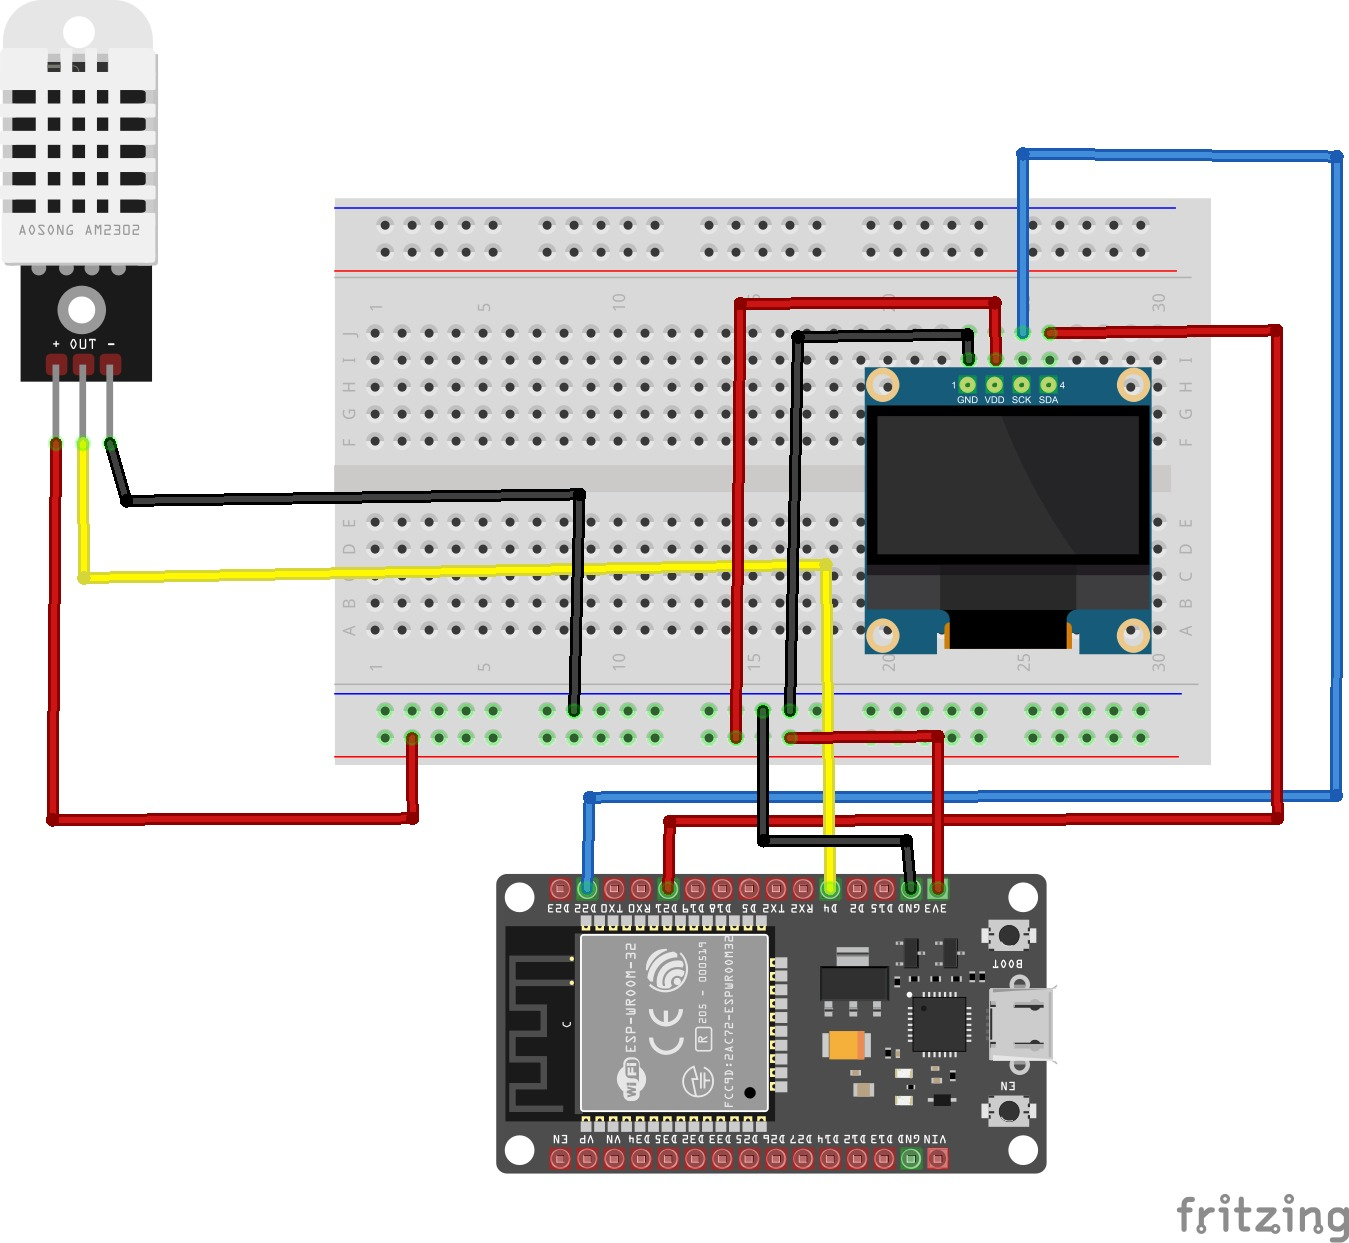
\includegraphics[width=0.85\textwidth]{../Esquemas/Temperatura_esq.jpeg}
\caption{Esquema de conexión del circuito Temperatura sin Termómetro (Fritzing)}
\label{fig:esquema}
\end{figure}

\subsection{Descripción de las Conexiones}

\subsubsection*{Conexiones del Sensor DHT22}
\begin{enumerate}
    \item \textbf{Pin + (VCC)} del DHT22 se conecta al bus de 3.3V del ESP32 (cable rojo).
    \item \textbf{Pin OUT (Datos)} del DHT22 se conecta al \textbf{GPIO4} (D4) del ESP32 (cable amarillo).
    \item \textbf{Pin -- (GND)} del DHT22 se conecta al bus de tierra GND (cable negro).
\end{enumerate}

\subsubsection*{Conexiones de la Pantalla OLED}
\begin{enumerate}
    \item \textbf{GND} de la OLED se conecta al bus de tierra GND.
    \item \textbf{VDD} de la OLED se conecta al bus de 3.3V.
    \item \textbf{SCK (SCL)} de la OLED se conecta al \textbf{GPIO22} del ESP32 (línea de reloj I2C).
    \item \textbf{SDA} de la OLED se conecta al \textbf{GPIO21} del ESP32 (línea de datos I2C).
\end{enumerate}

\subsection{Diagrama de Conexiones Simplificado}
\begin{center}
\begin{tabular}{lll}
\toprule
\textbf{Componente} & \textbf{Pin} & \textbf{ESP32 GPIO} \\
\midrule
DHT22 & OUT (datos) & GPIO4 \\
DHT22 & VCC (+) & 3.3V \\
DHT22 & GND (--) & GND \\
OLED SSD1306 & SDA & GPIO21 \\
OLED SSD1306 & SCK (SCL) & GPIO22 \\
OLED SSD1306 & VDD & 3.3V \\
OLED SSD1306 & GND & GND \\
\bottomrule
\end{tabular}
\end{center}

% ══════════════════════════════════════════════════════════════
\section{Código Fuente}
% ══════════════════════════════════════════════════════════════

A continuación se presenta el código completo del proyecto con explicación detallada de cada sección:

\subsection{Código Completo (Temperatura\_sin\_termometro.ino)}
\begin{lstlisting}[language=C++, title=Temperatura\_sin\_termometro.ino]
#include <Wire.h>
#include <Adafruit_GFX.h>
#include <Adafruit_SSD1306.h>
#include <DHT.h>

// ---------------------------
// Configuracion de la OLED
// ---------------------------
#define SCREEN_WIDTH 128
#define SCREEN_HEIGHT 64
#define OLED_RESET    -1

Adafruit_SSD1306 display(SCREEN_WIDTH, SCREEN_HEIGHT, &Wire, OLED_RESET);

// ---------------------------
// Configuracion del DHT
// ---------------------------
#define DHTPIN 4        // Pin D4 del ESP32 = GPIO 4
#define DHTTYPE DHT22

DHT dht(DHTPIN, DHTTYPE);

void setup() {
  Serial.begin(115200);

  // Inicia I2C con SDA=21 y SCL=22
  Wire.begin(21, 22);

  // Inicia pantalla OLED (direccion I2C: 0x7A)
  if (!display.begin(SSD1306_SWITCHCAPVCC, 0x7A)) {
    Serial.println("No se encontro la pantalla OLED");
    while (true);
  }

  // Inicia sensor DHT
  dht.begin();

  // Pantalla de inicio
  display.clearDisplay();
  display.setTextColor(SSD1306_WHITE);
  display.setTextSize(1);
  display.setCursor(0, 0);
  display.println("ESP32 + DHT + OLED");
  display.println("Iniciando...");
  display.display();

  delay(2000);
}

void loop() {
  // Espera entre lecturas del DHT
  delay(2000);

  float humedad = dht.readHumidity();
  float temperatura = dht.readTemperature(); // Celsius

  // Verifica si la lectura fallo
  if (isnan(humedad) || isnan(temperatura)) {
    Serial.println("Error al leer el sensor DHT");

    display.clearDisplay();
    display.setTextSize(1);
    display.setCursor(0, 0);
    display.println("Error al leer");
    display.println("el sensor DHT");
    display.display();
    return;
  }

  // Muestra en el monitor serial
  Serial.print("Temperatura: ");
  Serial.print(temperatura);
  Serial.println(" C");

  Serial.print("Humedad: ");
  Serial.print(humedad);
  Serial.println(" %");

  // Muestra en la OLED
  display.clearDisplay();

  display.setTextSize(1);
  display.setCursor(0, 0);
  display.println("Lectura ambiental");

  display.setTextSize(2);
  display.setCursor(0, 20);
  display.print(temperatura, 1);
  display.println(" C");

  display.setCursor(0, 45);
  display.print(humedad, 1);
  display.println(" %");

  display.display();
}
\end{lstlisting}

% ══════════════════════════════════════════════════════════════
\subsection{Análisis del Código}
% ══════════════════════════════════════════════════════════════

\subsubsection*{Librerías Incluidas}
El programa utiliza cuatro librerías externas:
\begin{itemize}
    \item \textbf{\texttt{Wire.h}:} Librería nativa de Arduino para comunicación I2C. Gestiona las líneas SDA y SCL.
    \item \textbf{\texttt{Adafruit\_GFX.h}:} Librería gráfica base de Adafruit que proporciona primitivas de dibujo (texto, líneas, rectángulos, círculos).
    \item \textbf{\texttt{Adafruit\_SSD1306.h}:} Driver específico para pantallas OLED con controlador SSD1306. Hereda de \texttt{Adafruit\_GFX}.
    \item \textbf{\texttt{DHT.h}:} Librería para sensores de la familia DHT (DHT11, DHT21, DHT22). Maneja el protocolo de comunicación propietario.
\end{itemize}

\subsubsection*{Constantes y Objetos}
\begin{itemize}
    \item \textbf{\texttt{SCREEN\_WIDTH} y \texttt{SCREEN\_HEIGHT}:} Definen la resolución de la OLED (128$\times$64 píxeles).
    \item \textbf{\texttt{OLED\_RESET = -1}:} Indica que la pantalla no usa un pin de reset dedicado (comparte el reset del ESP32).
    \item \textbf{\texttt{DHTPIN = 4}:} El pin GPIO4 del ESP32 se usa para la comunicación con el DHT22.
    \item \textbf{\texttt{DHTTYPE = DHT22}:} Selecciona el tipo de sensor. Cambiar a \texttt{DHT11} si se usa ese modelo.
    \item Se crean dos objetos: \texttt{display} (pantalla OLED) y \texttt{dht} (sensor de temperatura/humedad).
\end{itemize}

\subsubsection*{Función \texttt{setup()}}
Se ejecuta una sola vez al iniciar el ESP32 y realiza la inicialización completa del sistema:

\begin{enumerate}
    \item \textbf{\texttt{Serial.begin(115200)}:} Inicia la comunicación serial a 115200 baudios para depuración.
    \item \textbf{\texttt{Wire.begin(21, 22)}:} Inicializa el bus I2C especificando SDA en GPIO21 y SCL en GPIO22 (pines por defecto del ESP32).
    \item \textbf{Inicialización de la OLED:} \texttt{display.begin()} intenta comunicarse con la pantalla en la dirección I2C \texttt{0x7A}. Si falla, imprime un mensaje de error y detiene el programa con un bucle infinito.
    \item \textbf{\texttt{dht.begin()}:} Inicializa el sensor DHT22 configurando el pin y los tiempos de comunicación.
    \item \textbf{Pantalla de inicio:} Muestra el mensaje ``ESP32 + DHT + OLED / Iniciando...'' durante 2 segundos como retroalimentación visual al usuario.
\end{enumerate}

\subsubsection*{Función \texttt{loop()}}
Se ejecuta en ciclo infinito y contiene la lógica principal de lectura y visualización:

\begin{enumerate}
    \item \textbf{\texttt{delay(2000)}:} Espera 2 segundos entre lecturas, respetando el tiempo mínimo de muestreo del DHT22.
    \item \textbf{Lectura del sensor:} \texttt{dht.readHumidity()} y \texttt{dht.readTemperature()} obtienen las lecturas. Internamente, la librería envía una señal de inicio al DHT22, espera la respuesta de 40 bits (16 de humedad + 16 de temperatura + 8 de checksum) y decodifica los valores.
    \item \textbf{Verificación de errores:} La función \texttt{isnan()} comprueba si las lecturas son válidas. Si el sensor no responde o hay un error de comunicación, las funciones retornan \texttt{NaN} y el programa muestra un mensaje de error tanto en serial como en la OLED.
    \item \textbf{Salida serial:} Los valores se imprimen en el Monitor Serial con formato legible.
    \item \textbf{Visualización en OLED:} Se limpia la pantalla, se escribe el título ``Lectura ambiental'' en tamaño pequeño, y luego la temperatura y humedad en tamaño grande (2x) para fácil lectura a distancia.
\end{enumerate}

% ══════════════════════════════════════════════════════════════
\section{Principio de Funcionamiento}
% ══════════════════════════════════════════════════════════════

\subsection{Comunicación con el Sensor DHT22}
El DHT22 utiliza un protocolo propietario de un solo hilo (\textit{single-wire}) para transmitir datos. El proceso de lectura consiste en:

\begin{enumerate}
    \item El ESP32 envía una señal de inicio: pone la línea de datos en \texttt{LOW} durante al menos 1\,ms, luego la libera.
    \item El DHT22 responde con una señal de confirmación (\texttt{LOW} 80\,$\mu$s + \texttt{HIGH} 80\,$\mu$s).
    \item El sensor transmite 40 bits de datos secuencialmente: cada bit comienza con \texttt{LOW} (50\,$\mu$s) seguido de \texttt{HIGH}. La duración del pulso alto determina el valor: 26--28\,$\mu$s = bit ``0'', 70\,$\mu$s = bit ``1''.
    \item Los 40 bits se distribuyen así: 16 bits de humedad, 16 bits de temperatura y 8 bits de checksum.
\end{enumerate}

\subsection{Comunicación I2C con la Pantalla OLED}
El protocolo I2C (\textit{Inter-Integrated Circuit}) utiliza dos líneas:
\begin{itemize}
    \item \textbf{SDA (Serial Data):} Línea bidireccional de datos (GPIO21).
    \item \textbf{SCL (Serial Clock):} Línea de reloj generada por el maestro (GPIO22).
\end{itemize}

El ESP32 actúa como \textit{maestro} y la pantalla OLED como \textit{esclavo} con dirección \texttt{0x7A}. Los comandos y datos de píxeles se envían mediante tramas I2C que incluyen: condición de inicio, dirección del esclavo, byte de control (comando o datos) y los bytes de información.

\subsection{Conversión de Temperatura}
El sensor DHT22 contiene internamente un termistor NTC (\textit{Negative Temperature Coefficient}) y un sensor capacitivo de humedad. El termistor varía su resistencia con la temperatura según la relación:

\begin{equation}
R(T) = R_0 \cdot e^{\beta\left(\frac{1}{T} - \frac{1}{T_0}\right)}
\label{eq:steinhart}
\end{equation}

donde $R_0$ es la resistencia a la temperatura de referencia $T_0$ (generalmente 25$\,^\circ$C) y $\beta$ es la constante del material. El circuito interno del DHT22 realiza esta conversión y entrega directamente el valor digital de temperatura en grados Celsius.

% ══════════════════════════════════════════════════════════════
\section{Fotografía del Montaje}
% ══════════════════════════════════════════════════════════════

La siguiente imagen muestra el proyecto montado y en funcionamiento. Se puede observar el ESP32 conectado al computador vía USB, el sensor DHT22 a la izquierda, y la pantalla OLED mostrando los valores de temperatura y humedad. En la pantalla del computador se aprecia la terminal del Arduino IDE confirmando la carga exitosa del firmware.

\begin{figure}[H]
\centering

\includegraphics[width=0.7\textwidth]{../Imagenes/Temperatura_sin_termometro_img/Temperatura_sin_termometro.jpeg}
\caption{Montaje físico del proyecto Temperatura sin Termómetro}
\label{fig:montaje}
\end{figure}

% ══════════════════════════════════════════════════════════════
\section{Proceso de Creación}
% ══════════════════════════════════════════════════════════════

El desarrollo de este proyecto siguió los siguientes pasos:

\begin{enumerate}
    \item \textbf{Selección de componentes:} Se eligió el sensor DHT22 por su buena precisión y facilidad de uso. La pantalla OLED SSD1306 fue seleccionada por su bajo consumo, excelente contraste y comunicación I2C (solo 2 cables de datos).
    
    \item \textbf{Diseño del circuito:} Se diseñó el esquema en Fritzing conectando el DHT22 al GPIO4 y la OLED al bus I2C (GPIO21/GPIO22). Ambos dispositivos se alimentan a 3.3V desde el ESP32.
    
    \item \textbf{Instalación de librerías:} En el Arduino IDE se instalaron las librerías necesarias desde el Gestor de Librerías:
    \begin{itemize}
        \item \texttt{Adafruit SSD1306} (para la pantalla OLED)
        \item \texttt{Adafruit GFX Library} (gráficos base)
        \item \texttt{DHT sensor library} de Adafruit (para el sensor)
    \end{itemize}
    
    \item \textbf{Montaje en protoboard:} Se conectaron los componentes siguiendo el esquema de la Figura~\ref{fig:esquema}.
    
    \item \textbf{Desarrollo del firmware:} Se escribió el código en el Arduino IDE, implementando la lectura del sensor cada 2 segundos y la visualización dual (serial + OLED).
    
    \item \textbf{Configuración del Arduino IDE:}
    \begin{itemize}
        \item Placa seleccionada: \textit{ESP32 Dev Module}.
        \item Velocidad de subida: 115200 baudios.
        \item Puerto: COM correspondiente al ESP32 conectado.
    \end{itemize}
    
    \item \textbf{Calibración de la dirección I2C:} Se verificó la dirección I2C de la pantalla OLED. En este caso, la dirección resultó ser \texttt{0x7A} (puede variar según el fabricante; valores comunes son \texttt{0x3C} y \texttt{0x3D}).
    
    \item \textbf{Pruebas y validación:} Se verificaron las lecturas comparándolas con un termómetro de referencia, confirmando la precisión del sensor DHT22.
\end{enumerate}

% ══════════════════════════════════════════════════════════════
\section{Conclusiones}
% ══════════════════════════════════════════════════════════════

\begin{itemize}
    \item El proyecto demuestra cómo obtener mediciones ambientales precisas utilizando componentes electrónicos digitales de bajo costo, sin necesidad de instrumentos analógicos tradicionales.
    \item El sensor DHT22 proporciona lecturas confiables de temperatura ($\pm 0.5\,^\circ$C) y humedad ($\pm 2$--$5$\%), adecuadas para la mayoría de aplicaciones domésticas y educativas.
    \item La pantalla OLED SSD1306 permite una visualización clara y autónoma de los datos, eliminando la dependencia del computador una vez cargado el firmware.
    \item La comunicación I2C simplifica el cableado al requerir solo dos líneas de datos para controlar la pantalla, dejando más pines GPIO disponibles para otros periféricos.
    \item El manejo de errores con \texttt{isnan()} asegura que el sistema informe al usuario cuando el sensor no responde, mejorando la robustez del sistema.
    \item Este proyecto constituye la base para sistemas de monitoreo ambiental más avanzados, como estaciones meteorológicas con registro de datos, alertas por Wi-Fi, o integración con plataformas IoT como ThingSpeak o Blynk.
\end{itemize}

\end{document}
